\documentclass{article}
\usepackage{amssymb}% http://ctan.org/pkg/amssymb
\usepackage{pifont}% http://ctan.org/pkg/pifont
\newcommand{\cmark}{\ding{51}}%
% Updated definition, see explanation below
\newcommand*{\fullref}[1]{\hyperref[{#1}]{\autoref*{#1} \nameref*{#1}}} % One single link
\usepackage{geometry}
\usepackage{parskip}
\usepackage{pdflscape}
\usepackage{lscape}
\usepackage[colorlinks,pdfpagelabels,pdfstartview = FitH,bookmarksnumbered = true,linkcolor = black,citecolor = black]{hyperref}		% Inhaltsverzeichnis anklickbar
\usepackage{scrpage2} 									% Kopf- und Fusszeile
\pagestyle{scrheadings}
\renewcommand{\headfont}{\small}
\ihead{
\includegraphics[width=3cm]{NTB-FHO_LOGO}} % Kopfzeile links
\setlength{\headsep}{18mm}
\ohead{xl2DB}												 % Kopfzeile rechts
\ifoot{} 													 % Fusszeile links
\cfoot{\thepage}					 							     % Fusszeile mitte
\ofoot{}													 % Fusszeile rechts
\setheadsepline{0.4pt}										 % fügt horizontale linie ein 
\usepackage[utf8]{inputenc}
\usepackage[T1]{fontenc}
\usepackage{color}
\usepackage{lmodern} % load a font with all the characters
\usepackage{graphicx}
\usepackage{caption}
\usepackage{subcaption}
\usepackage{enumitem}
\usepackage{titlesec}	
\setlist[description]{leftmargin=\parindent,labelindent=\parindent}
\graphicspath{{Bilder/}}
\geometry{
	a4paper,
	total={210mm,297mm},
	left=25mm,
	right=25mm,
	top=28mm,
	bottom=25mm
}
\definecolor{carrotorange}{rgb}{0.93, 0.57, 0.13}
\renewcommand{\contentsname}{Inhaltsverzeichnis}
\renewcommand{\listfigurename}{Abbildungsverzeichnis}
\renewcommand{\figurename}{Bild}


%%%%%%%%%%%%%%%%%%%%%%%%%%% BEGIN %%%%%%%%%%%%%%%%%%%%%%%%%%%%%%%%%%

\begin{document}
\section*{\centering Bedienungsanleitung  - xl2DB}
\subsection*{Installation}
Für die Installation der Software muss man nur die Datei "setup.exe" ausführen die sich im Installations Ordner befindet und bei jeweiligen Aufforderungen auf "Ok", "Ja" oder ähnliches drücken.

\subsection*{Excel File Vorbereitung}
Das format des Excel Files muss wie im Bild 1. unten aussehen (ID, Anrede, Nachname usw. muss genau so geschrieben werden): 
\begin{figure}[h]
	\begin{center}
		\centering
		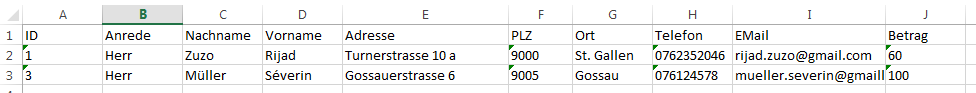
\includegraphics[width=0.8\paperwidth]{vorlageExcel}
		\caption{Excel Vorlage}
	\end{center}
\end{figure}

Und die aktuelle Tabelle im Excel File muss wie im Bild 2. unten benannt werden: 
\begin{figure}[h]
	\begin{center}
		\centering
		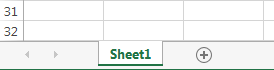
\includegraphics[width=0.3\paperwidth]{vorlageExcelSheet1}
		\caption{Excel Vorlage}
	\end{center}
\end{figure}

Falls dies nicht gemacht wird, werden einige Funktionen der Applikation nicht wie erwünscht Funktionieren. Wenn deer Tabellenname nicht in "Sheet1" geändert wird wird die Verbindung zum Excel File unmöglich.

\subsection*{Ausführung}
Nach der erfolgreichen Installation sollte auf dem Desktop das Icon mit dem name xl2DB.exe auftauchen und die Applikation wird sofort nach der Installation automatisch aufgerufen.

\begin{figure}[h]
	\begin{center}
		\centering
		
\includegraphics[width=0.1\paperwidth]{Icon}
		\caption{xl2DB.exe Icon}
	\end{center}
\end{figure}

Bei dem ersten Aufruf der Applikation erscheint ein "Wilkommen" Fenster und die Applikation ist bereit zur Nutzung.

\newpage

\subsection*{Erste schritte}
Wenn die Applikation das erste mal aufgerufen wurde, muss man im oberen linken Teil in dem Menü Streifen den Datenbankpfad (Excel File Pfad) setzten und dieser wird intern gespeichert. Bei dem nächsten Aufruf der Applikation wird dieser Pfad automatisch geladen. 

\begin{figure}[h]
	\begin{center}
		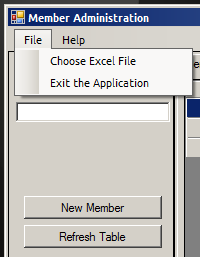
\includegraphics[width=0.2\paperwidth]{Pfads}
		\caption{Menü Streifen Excel File Auswahl}
	\end{center}
\end{figure}

Es wird ein Filechooser Fenster geöffnet wie unten im Bild 5. :
\begin{figure}[h]
	\begin{center}
		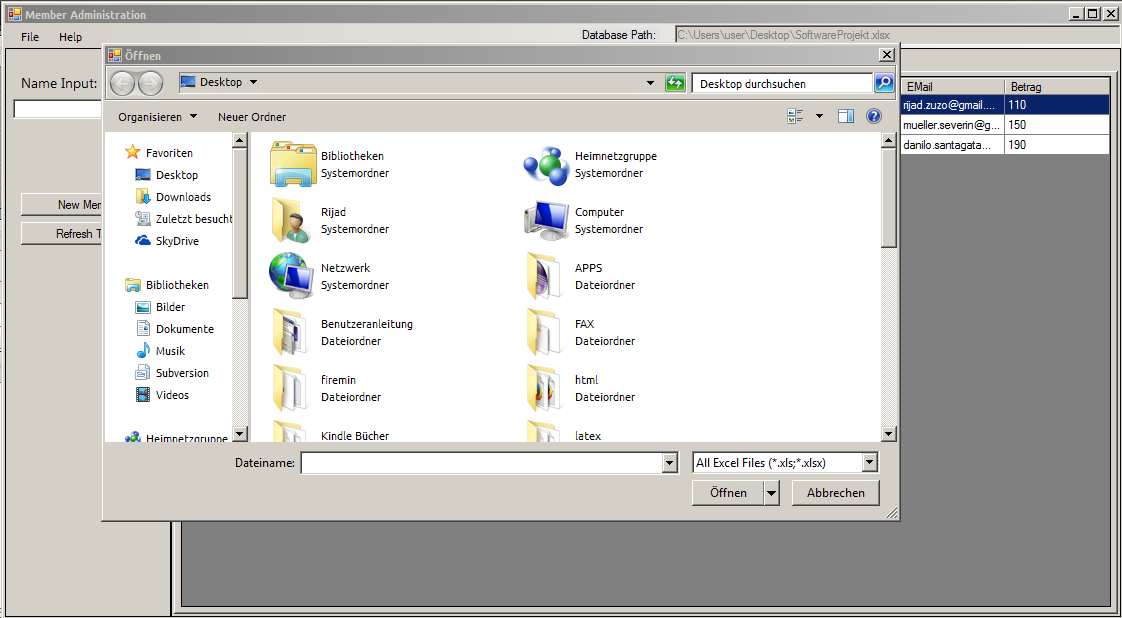
\includegraphics[width=0.8\paperwidth]{Filechooser}
		\caption{Filechooser Fenster}
	\end{center}
\end{figure}

Hier kann man leicht zu einem gewünschten Dokument navigieren und diesen durch doppelklick oder auswählen und auf "Öffnen" drücken auswählen. Nach dem Auswählen der Datei schliesst sich dieses Fenster automatisch und die Daten werden aus diesem File gezogen und in der Tabelle Bild 6. dargestellt.

\newpage

\begin{figure}[h]
	\begin{center}
		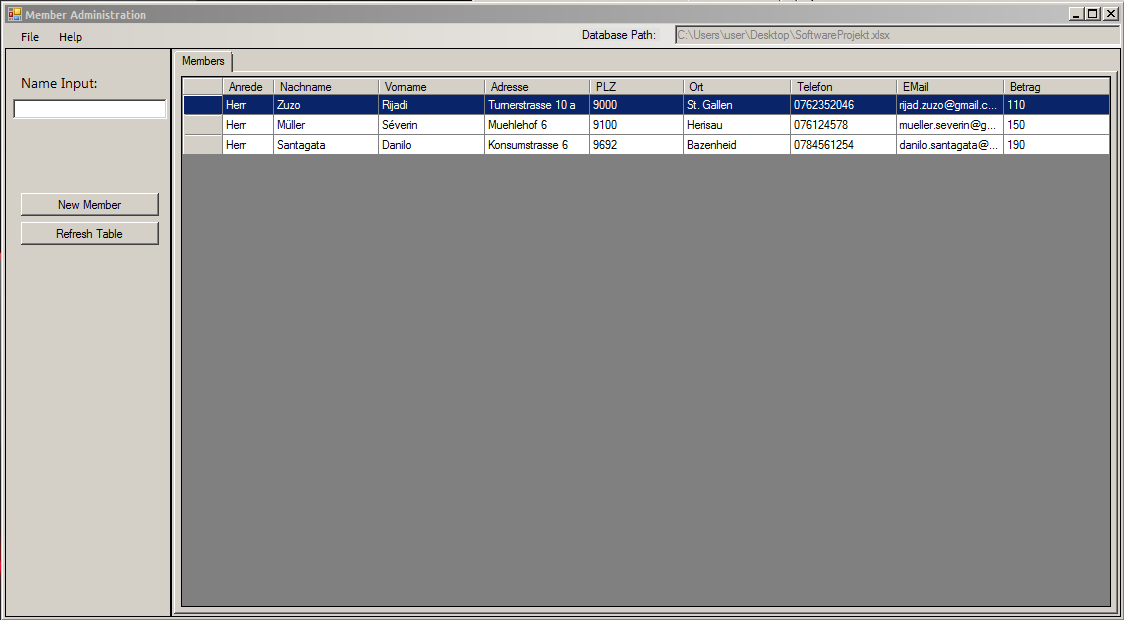
\includegraphics[width=0.8\paperwidth]{printscreen}
		\caption{Geladene Daten in Tabelle}
	\end{center}
\end{figure}

Jetzt ist die Applikation bereit für weitere Aktionen, die eigentlich recht intuitiv sind und bedürfen kein weiteres erklären. 

Zusammengefasst: 
\begin{itemize}
\item Ein klick auf "New Member" erzeugt das Formular für das Eingeben der Daten bei erstellen eines neuen Mitglieds (Bild 7.a).
 
\item Ein klick in der Tabelle auf eine Zeile öffnet das "PersonWindow" mit allen Informationen betreffend der angeklickten Zeile (Bild 7.b). In diesem Fenster kann man Änderungen vornehmen und speichern oder Mitglieder ganz löschen.
\end{itemize}

 \begin{figure}[h]
 	\centering
 	\begin{subfigure}{.4\textwidth}
 		\centering
 		\includegraphics[width=.7\linewidth]{NewMemberGui}
 		\caption{Neues Mitglied Formular}
 		\label{fig:sub1}
 	\end{subfigure}%
 	\begin{subfigure}{.5\textwidth}
 		\centering
 		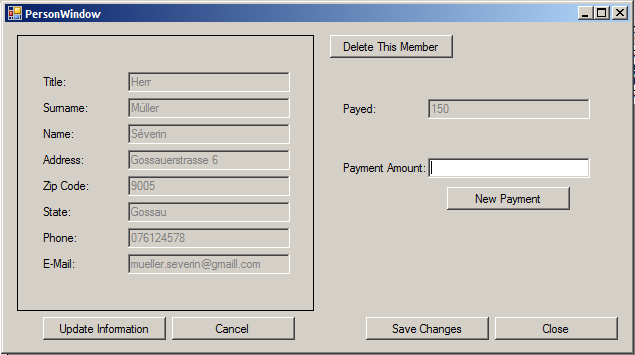
\includegraphics[width=.9\linewidth]{MemberInfoGUI}
 		\caption{Mitgliedsinformation Fenster}
 		\label{fig:sub2}
 	\end{subfigure}
 	\caption{Aufrufbare Fenster}
 	\label{fig:test}
 \end{figure}
 
 \centering \large Wir wünschen viel Spass und Erfolg bei der Nutzung unserer Software. 
\end{document}